\documentclass[addpoints]{exam}
\usepackage{amsmath}
\usepackage{amsfonts}
\usepackage{tcolorbox}
\usepackage{tikz}
\usepackage{pgfplots}
\usepackage{mdframed}
\usepackage{hyperref}

% externalize figures to optimize compile time
\usepgfplotslibrary{external}
\tikzexternalize

\hypersetup{
    colorlinks=true,
    linkcolor=blue,
    filecolor=magenta,      
    urlcolor=blue,
    pdfpagemode=FullScreen,
    }

\urlstyle{same}
%=============================================
        %POINTS FORMATTING
%=============================================
\marksnotpoints 
%if you would prefer the exam to say "points" instead of "marks", you can delete the above line.

%\pointformat{\textbf{(\thepoints)}} 
%delete comment if you want bold points

\pointsinrightmargin
%\marginpointname{ \points}
\bracketedpoints
%delete comment if you want point values to be printed in the right margin instead of at the start of the question. The same command with the "right" places the point values on the left margin.

%\
%=============================================
        %HEADER/FOOTER FORMATTING
%=============================================
\pagestyle{headandfoot}
\firstpageheadrule
\runningheadrule
\firstpageheader{Unit 7: Sequences and Series}{Lagrange Error}{Shah \\ BC Calc}
\runningheader{Unit 7}{LEB}{BC Calc}
\firstpagefooter{}{}{}
\runningfooter{ }{\thepage}{ }

\begin{document}

\vspace{1in}

\begin{tcolorbox}[title=TAYLOR POLYNOMIALS REVIEW ,colframe=black,sharp corners,colback=white,colbacktitle=white,coltitle=black]
   Before we talk about Lagrange Error (also known as Taylor's Theorem) lets do a quick recap of Taylor polynomials. Taylor polynomials are polynomials that we can use to approximate transcendental functions like $e^x \text{ and } \sin x$. If there is some function $f$ that has $n$ derivatives then,
   \[\displaystyle
   P_n(x) = f(c) + f'(c)\left(x-c\right) + \frac{f''(c)}{2\textbf{!}}\left(x-c\right)^2+ \frac{f'''(c)}{3\textbf{!}} \left(x-c\right)^3 + \dots + \frac{f^{\left(n\right)}(c)}{n\textbf{!}}\left(x-c\right)^n
   \]
    is the $n$th Taylor Polynomial for $f$ centered around $c$. \\
    \textit{* Note that in the special case where $c=0$ the polynomial is known as the Maclaurin Polynomial} \\
    Now as we increase the degree of the Taylor polynomial we can increase the accuracy of our approximation of our function. 

    \vspace{0.3in}

    \begin{minipage}{0.45\linewidth}
        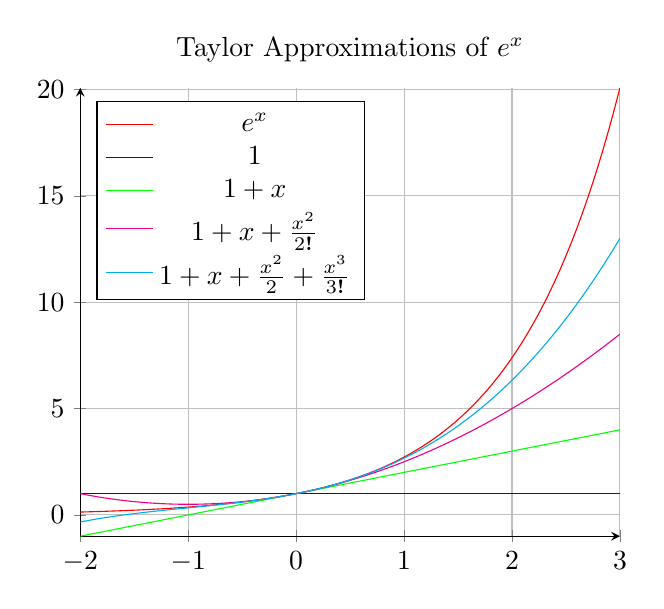
\begin{tikzpicture}
            \begin{axis}[
            title=Taylor Approximations of $e^x$,
            legend pos = north west,
            axis lines = left, 
            grid=major,
            ]
    
            \addplot[
            domain=-2:3,
            samples=100,
            color=red
            ]{e^x};
            \addlegendentry{\(e^x\)}
    
            \addplot[
            domain=-2:3,
            samples=100,
            color=blue
            ]{1};
            \addlegendentry{\(1\)};
            
            \addplot[
            domain=-2:3,
            samples=100,
            color=green
            ]{x+1};
            \addlegendentry{\(1+x\)};
            
            \addplot[
            domain=-2:3,
            samples=100,
            color=magenta
            ]{1+x+x^2/2};
            \addlegendentry{\(1+x+\frac{x^2}{2\textbf{!}}\)};
    
            \addplot[
            domain=-2:3,
            samples=100,
            color=cyan
            ]{1+x+x^2/2+x^3/6};
            \addlegendentry{\(1+x+\frac{x^2}{2}+\frac{x^3}{3\textbf{!}}\)};
                
            \end{axis}
        \end{tikzpicture}
    \end{minipage}
    \hfill
    \begin{minipage}{0.45\linewidth}
        The graph to the left shows the first 4 terms of the Maclaurin polynomial for $e^x$. The key thing to note here is that as the polynomial increases in degree (\textcolor{blue}{blue} $\rightarrow$ \textcolor{green}{green} $\rightarrow$ \textcolor{violet}{violet} $\rightarrow$ \textcolor{cyan}{cyan}) the polynomial more closely approximates $e^x$. This is the key idea that we will use to in the calculation of our Lagrange Error Bound\footnote[1]{\href{https://www.desmos.com/calculator/tblpvqcvdx}{\underline{See this desmos demo for more}}}. 
        \vspace{0.1in}
        \newline
        Also notice that because this polynomial was centered around $0$, we named it the MacLaurin polynomial for $e^x$
    \end{minipage}
\end{tcolorbox}

\begin{tcolorbox}[title=TAYLOR'S THEOREM (LAGRANGE ERROR) ,colframe=black,sharp corners,colback=white,colbacktitle=white,coltitle=black]
    Before we talk about how to find the lagrange error lets first think about what the lagrange error bound is \textit{used} for.
    \vspace{0.1in}
    \newline
    Lets assume you have a function $f(x)$ and the $n$th degree taylor approximation of $f$ centered around $c$, $P_n(x)$. Now lets say that you want to approximate the value of $f$ at some value $x=z$, so you find the value of $P_n(z)$. Now remembering that $P_n$ is only an approximation you want to find the error in your approximation. \textbf{This is what Taylor's Theorem tells us.}
    \vspace{0.1in}
    \newline
    Just like the alternating series remainder theorem the Lagrange error bound will utilize the next omitted term to find the remainder between your approximation and the real value, in our case, this next neglected term will be the next higher derivative. This makes sense if you recall from the recap section where above we stated that as we increased the number of derivatives, our approximation (Taylor) polynomial got better and more accurate. Now you might be tempted to immediately calculate the $n+1$th Taylor polynomial, $P_{n+1}$ and evaluate it at $z$; however, just like in the alternating series remainder theorem we will be focusing on the next neglected \underline{term}. 
    \end{tcolorbox}
    
\begin{tcolorbox}[title=TAYLOR'S THEOREM (LAGRANGE ERROR) (cont.) ,colframe=black,sharp corners,colback=white,colbacktitle=white,coltitle=black]
    With this lets (let's?) start constructing our formula:
    \[\displaystyle
        R_n(x) = \frac{f^{\left(n+1\right)}\left(x-c\right)}{\left(n+1\right)\textbf{!}}\left(x-c\right)^{n+1} \hspace{0.1in} \text{where $R_n(x)$ is our remainder function}
    \]
    Hopefully, you'll recognize this as the $n+1$th term of our Taylor polynomial $P_n$. Now there are a few small tweaks we can make to this formula to help us find a better error bound.
    \vspace{0.1in}
    \newline
    First start by considering what this formula tells us in its current state: the remainder (or error), $R_n$ is \textit{exactly} equal to the next neglected term (or next higher derivative). Now while this is nice we want to cover all our bases, so instead of seeking the exact error, lets find the \textbf{maximum} error that could possible occur with our approximation. We can start by turning this into an inequality:
    \begin{equation*}
        R_n(x) \leq \frac{f^{\left(n+1\right)}\left(x-c\right)}{\left(n+1\right)\textbf{!}}\left(x-c\right)^{n+1} \hspace{0.1in} \text{where $R_n(x)$ is our remainder function}
    \end{equation*}
    Then we can focus on making our function as large as possible. We will do this in two steps:
    \begin{equation}\label{eq:1}
        R_n(x) \leq \left| \frac{f^{\left(n+1\right)}\left(z\right)}{\left(n+1\right)\textbf{!}}\right|\left|x-c\right|^{n+1} \hspace{0.1in} \text{where $R_n(x)$ is our remainder function}
    \end{equation}
    \begin{equation}\label{eq:2}
        R_n(x) \leq \textbf{max}\left| \frac{f^{\left(n+1\right)}\left(z\right)}{\left(n+1\right)\textbf{!}}\right|\left|x-c\right|^{n+1} \hspace{0.1in} \text{where $R_n(x)$ is our remainder function}
    \end{equation}
    To maximize the value of our function we first added absolute value bars in equation (\ref{eq:1}). Then we physically maximized the function by taking the maximum value of $f^{\left(n+1\right)}$ with the \textbf{max} function, as seen in equation (\ref{eq:2}). There are a few things to note here:
    \begin{enumerate}
        \item $z$ is going to be a number between $x$ and $c$.
        \item $n$ is simply the $n$th derivative of our \textit{original} function. It is very important to note that $n$ comes from the original polynomial and not the one used to find error. 
        \item $c$ is the center of the taylor polynomial.
        \item $x$ is the value we are trying to approximate.
        \item $\textbf{max}\left|f^{\left(n+1\right)}\right|$ is the maximum possible value of $f^{\left(n+1\right)}$ at $z$. Often times you won't know what this is so you'll have to guess what this is (we'll talk about this in a minute).
    \end{enumerate} 
    You'll also note that we are now evaluating the $n+1$th derivative at $z$ instead of $x-c$. This is because we want the maximum value of the derivative at whatever point we are approximating so we choose some number $z$ to represent the function input that gives us the maximum value. 
    \vspace{0.1in}
    \newline
    As for actually finding $\textbf{max}\left|f^{\left(n+1\right)}\right|$ there are a few tricks we can use. If our \textit{original} function is a trig function, then we can immediately assume that $1$ is our maximum value. This is because $0\leq \sin, \cos, \tan, \leq 1$. In other scenarios when we are not dealing with trig functions we can use logic to deduce a good maximum value. For example, if $f^n(x)=n^n$ and the original Taylor polynomial is 3 terms long ($n=3$) then using $\left(n+1\right)^{\left(n+1\right)}=4^4$ would be a good choice because we know that it \textit{must} be larger than the $n$th derivative evaluated at that same point. Or, for instance, if our original function was $\textbf{e}^x$ then we know that if $c \leq z \leq x$ that $e^x$  (where $x$ is the number we are approximating the value of) is a good assumption for the max value. The main thing to keep in mind is that the closer your max value is the better your error approximation will be.
\end{tcolorbox}
\end{document}